\documentclass{style/notices}
\usepackage{amsfonts,amssymb,amsmath,amscd,amsthm}
\usepackage{graphicx}
\usepackage{xcolor}
\usepackage{cleveref}
\usepackage{float}
\usepackage{xr-hyper}
\usepackage{hyperref}
\hypersetup{pdfborder = 0 0 0}

\title{
    Measuring Diversity and Segregation with Convex Functions
}

\author{
  Philip S. Chodrow
  \affil{
    Phil is an assistant professor of computer science at Middlebury College. His email address is \tt{pchodrow@middlebury.edu}.
    }
}


% abbreviations in the segregation chapter

\theoremstyle{definition}
\newtheorem{dfn}{Definition}

\newcommand{\N}{\mathbb{N}}
\newcommand{\R}{\mathbb{R}}



\newcommand{\simplex}[1]{\Delta_{#1}}
\newcommand{\paren}[1]{\left( #1 \right)}
\newcommand{\braces}[1]{\left\{ #1 \right\}}
\newcommand{\brackets}[1]{\left[ #1 \right]}
\newcommand{\vy}{\mathbf{y}}
\newcommand{\mX}{\mathbf{X}}
\newcommand{\mY}{\mathbf{Y}}
\newcommand{\mV}{\mathbf{V}}
\newcommand{\mU}{\mathbf{U}}
\newcommand{\cX}{\mathcal{X}}
\newcommand{\cP}{\mathcal{P}}
\newcommand{\scP}{\mathscr{P}}
\newcommand{\abs}[1]{\left| #1 \right|}
\newcommand{\norm}[1]{\lVert #1 \rVert}
\newcommand{\agg}[3]{\mathrm{agg}_{#1#2}\paren{#3}}
\newcommand{\mig}[4]{\mathrm{mig}_{#1,#2\rightarrow#3}^{(#4)}}
\newcommand{\exc}[5]{\mathrm{exc}_{#1,#2, #3\leftrightarrow#4}^{(#5)}}
\DeclareMathOperator*{\argmax}{argmax}
\DeclareMathOperator*{\argmin}{argmin}
\newcommand{\ve}{\mathbf{e}}
\newcommand{\indicator}[1]{\mathbb{1}\brackets{#1}}
\newcommand{\vv}{\mathbf{v}}
\newcommand{\vu}{\mathbf{u}}
\newcommand{\vzero}{\mathbf{0}}
\newcommand{\trace}[1]{\mathrm{trace}\;#1}
\newcommand{\cH}{\mathcal{H}}
\newcommand{\vdelta}{\boldsymbol{\delta}}

\newcommand{\Pops}{\mathcal{P}}

\renewcommand{\textfraction}{0.1} 
\renewcommand{\floatpagefraction}{0.8}

\begin{document}

\maketitle

We consider the problem of \emph{segregation measurement}. 
Colloquially, a population of individuals is segregated with repect to a given trait if individuals with different values of that trait tend to be separated from one another by geography, policy, or other social forces.
The segregation measurement problem is to construct compact, quantitative descriptions of the extent and structure of segregation in a given population. 
The purpose of such a measurement is often comparative--we aim to say that one population (say, a city) is more segregated, or differently segregated, than another. 
We'll focus here on the problem of \emph{spatial} segregation, in which individuals are assumed to be located space (often at their place of residence) and we seek to understand how the strongly the spatial distribution of individuals reflects their demographic traits.

\Cref{fig:checkerboard} provides a classical illustration, as well as a few of its complexities. 
In each of the four panels, individuals with demographic possible demographic traits $A$ or $B$ are arranged into a synthetic ``city.''
Panel (a) describes such a city in which only members of group $B$ are present; intuitively such a city cannot display spatial sorting between groups because there is only one group present. 
Our first intuitive insight is then that \emph{diversity is necessary for segregation}. 
Panel (b) shows that diversity, however, is not sufficient; if each group is represented uniformly across the map, then there is also no spatial segregation. 
Panels (c) and (d) do display spatial segregation, with each individual location containing a uniform population of either 100\% $A$ or 100\% $B$.
Since each panel contains the same number of locations dominated by each group, any measure of segregation which ``forgets'' the spatial structure of the population will assign the same value to both panels; such a measure may be considered \emph{aspatial}. 
The problem of constructing \emph{spatial} measures (which successfully distinguish between panels (c) and (d) in intuitive ways) has often been called the ``checkerboard problem'' in the quantitative sociology literature \cite{reardon3MeasuresSpatial2004}. 
To summarize, a \emph{diversity} measure can distinguish panels (a) and (b); an aspatial \emph{segregation} measure can distinguish both from panel (c), and a \emph{spatial} segregation measure can distinguish (d) from (c).

\begin{figure*}
  \centering
  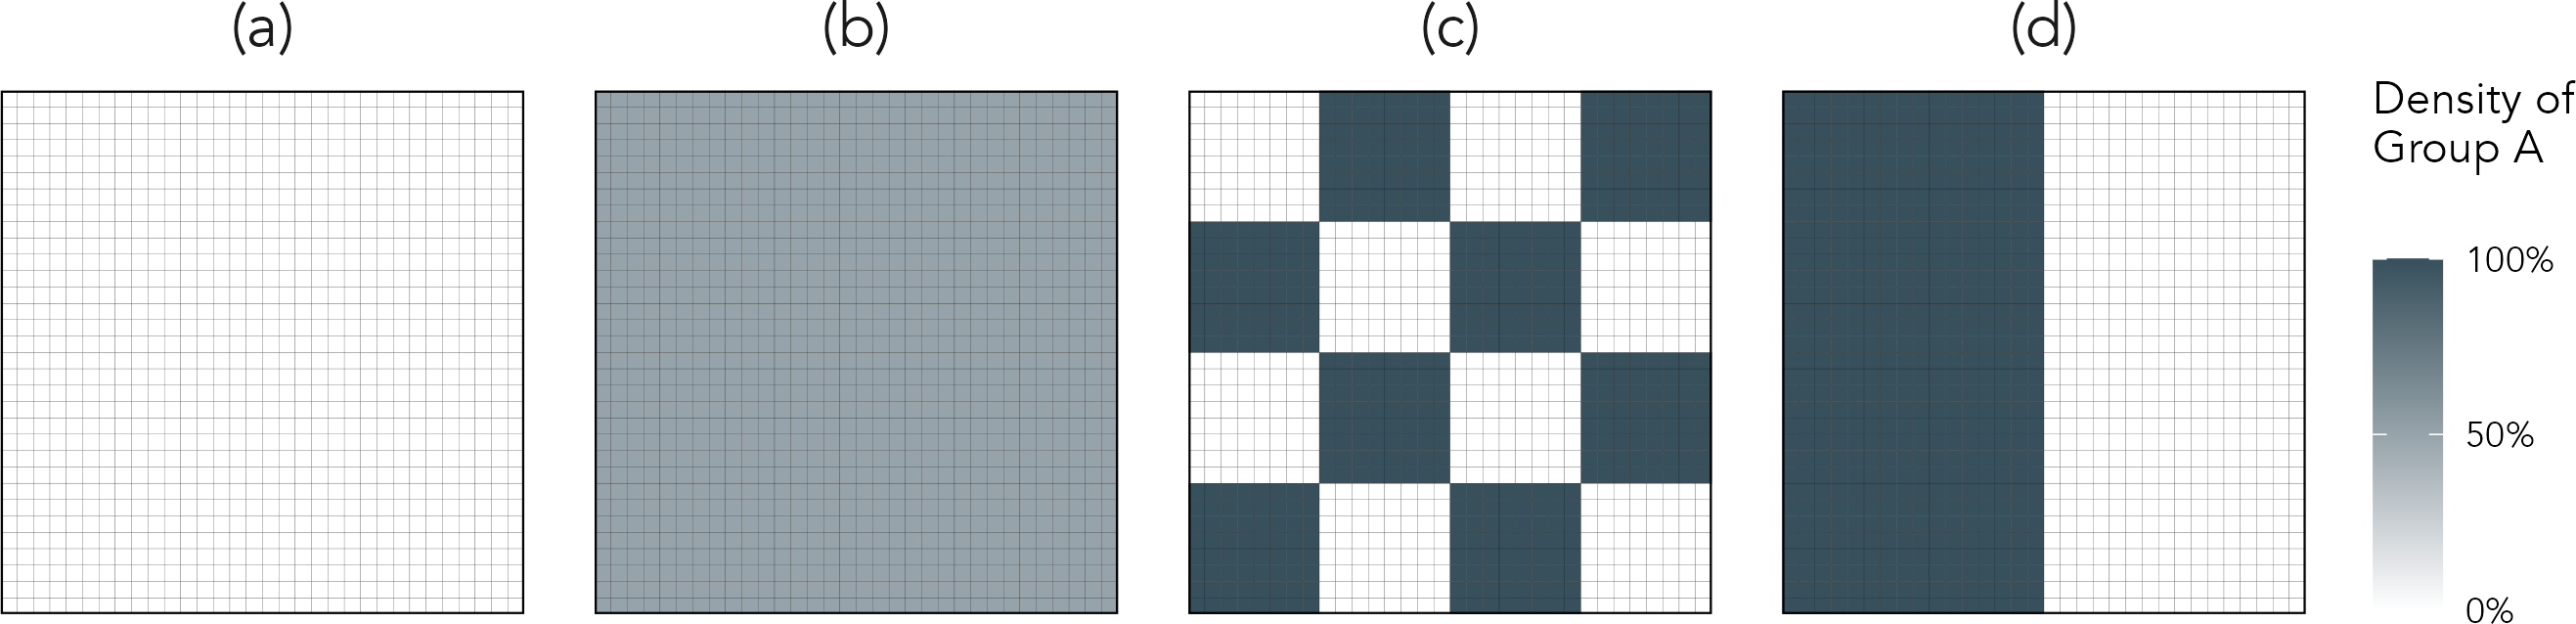
\includegraphics[width=1.0\textwidth]{fig/checkerboard.png}
  \caption{
    Synthetic ``cities'' composed of $\totalCellsPerSide{}\times \totalCellsPerSide{}$ spatial units. 
    Each contains an equal density of population, and individuals within the population may be of either group A (black) or group B (white). 
    Panel (c) is further arranged into \numBlocks{} blocks of \cellsPerBlock{} cells each.
    } \label{fig:checkerboard}
\end{figure*}


Any spatial measure which does successfully distinguish (c) and (d), however, is also subject to the \emph{modifiable areal unit problem (MAUP)} \cite{openshaw1984modifiable}: the method of aggregating continuous geographic space into discrete areal units (e.g. counties, tracts, blockgroups, or neighborhoods) is often arbitrary and can have a strong effect on the resulting segregation measurement.
By way of illustration, if in panel (c) the resolution of our measurement was coarsened to the scale of 16$\times$16 blocks, illustrated by the dark box, then we would be unable to distinguish (c) from (b). 

The study of quantitative measures for spatial segregation extends far enough back that a review article in 1955 could already express frustration and disappointment with the chaotic state of the methodology. 
Commenting then on the measures extant at the time, Duncan and Duncan \cite{duncanMethodologicalAnalysisSegregation1955} wrote: 
\begin{enumerate}
  \item \emph{The proposed indexes of segregation have a number of hitherto unnoticed interrelationships which can be mathematically demonstrated.} 
  \item \emph{Some of them have mathematical properties of which their proponents were unaware, and which lead to difficulties of interpretation.} 
  \item \emph{As a consequence, the status of the empirical work already done with segregation indices is questionable, and their validity for further research is undermined.} 
\end{enumerate}
Since that time, there have been efforts within quantitative sociology to impose a more unified mathematical structure on segregation measures, especially in the work of Sean Reardon and collaborators \cite{reardonMeasuresMultigroupSegregation2002, reardonMeasuresIncomeSegregation,,reardon3MeasuresSpatial2004}.
Still, over 70 years later, hints of the chaos described by Duncan and Duncan remain.
This author is aware of two instances within the last ten years of a diversity or segregation measure being published as novel despite already existing in the literature under a different name. 
Somewhat distinctly from the sociological literature, there has been some recent attention on segregation measurement in the mathematics community \cite{duchin2023measuring,topaz2025diversity,hoogstraQuantitativeMetricsTrait2025}. 
These works, though interesting and important in their own right, tend to be somewhat disconnected from recent progress within the sociology community. 

In this article, I argue that beginning with some of the systematic work in quantitative sociology not only enriches opportunities for conversation between mathematicians and social scientists but also provides a rich ground for interesting, accessible mathematics and data analysis. 
I do not attempt to offer a thorough review of prior work on segregation measurement, but rather offer my particular perspective and the sources which have informed it.
After establishing notation, we begin with a discussion of diversity measures, arguing that standard proposed axioms for these measures lead naturally to the class of convex functions defined on the probability simplex. 
Comparing global and average local diversities leads directly to a segregation measure interpretable as a measure of the information content that the spatial location carries about demographic information. 
We give several proofs showing that this general information measure satisfies many of the desirable properties of segregation measures proposed in the quantitative sociology literature. 
We then demonstrate two ways to ``spatialize'' this information, one using conditional information decomposition and another using the locally quadratic structure of Bregman divergences to construct a local measure of the spatial scale of segregation. 
We close with some discussion about extending this framework in the direction of ordinal segregation measures, as well as some open mathematical challenges.  

\section{Preliminaries} \label{sec:preliminaries}


  To make these ideas concrete, we formalize the idea of a \emph{population} and measurements which reflect the diversity or segregation of that population.  
  Our framework for defining populations is intentionally discrete, in recognition of the fact that all Census-type data sets provide demographic information in discrete areal units such as counties, tracts, or blockgroups. 

  \begin{dfn} \label{def:simplex}
      For $\ell \in \N,$ the \emph{probability simplex} $\simplex{\ell}$ is the set 
      \begin{align*}
          \simplex{\ell} = \braces{\vy \in \R^{\ell} : \sum_{j = 1}^{\ell} y_j = 1, y_j \geq 0 \text{ for all } j \in [\ell]}\;.
      \end{align*}
      of probability vectors on $\ell$ elements.\footnote{
        Although it is sometimes common to refer to $\simplex{\ell}$ as an $(\ell-1)$-simplex (this being its manifold dimension), we write $\simplex{\ell}$ to emphasize its role as the set of probability distributions over $\ell$ categories.
        } 
  \end{dfn}

  \begin{dfn} \label{def:population}
      A \emph{population} $\cP$ with $n$ locations in $d$ spatial dimensions and $\ell$ demographic categories is a triple $\cP = \paren{\mX, \mY, \mu}$, where: 
      \begin{itemize}
        \item $\mX \in \R^{n\times d}$ is a matrix with rows $\vx_i$, $i = 1, \ldots, n$.\footnote{$\mX$ can be replaced by a discrete metric space $(\cX, d)$ where $d$ describes measurement of distance between locations; under this replacement all the remaining results in this work hold except for \Cref{def:local-information,thm:local-information}.} 
        \item $\mY \in \R^{n \times \ell}$ is a row-stochastic matrix: for each row $i$, $\vy_i \in \simplex{\ell}$.
        \item $\mu \in \simplex{n}$.   
      \end{itemize}
      We denote the set of all populations with $n$ locations, $d$ dimensions, and $\ell$ demographic categories as $\Pops_{nd\ell}$. 
  \end{dfn}
  In this definition, the matrix $\mX$ represents space: element $\vx_i$ of $\mX$ can be viewed as giving the location of the $i$th spatial subunit of the population. 
  The matrix $\mY$ represents the demographic distribution of the population according to some attribute such as gender, race, or education level: the $i$th row $\vy_i$ of $\mY$ gives the proportion of individuals in each demographic category at location $i$.
  Finally, the probability vector $\mu$ represents the population density across locations; the proportion of individuals living in location $i$ is $\mu_i$. 
  The probability that a single individual, chosen uniformly at random from the population, lives in location $i$ and is in demographic category $j$ is $\mu_i y_{ij}$. 
  The mean population vector $\bar{\vy} = \sum_{i = 1}^n \mu_i \vy_i$ has entries giving the marginal probabilities that an individual chosen uniformly at random belongs to each demographic category. 
  \begin{dfn} \label{def:population-measurement}
    A \emph{population measurement} is a function $f: \Pops_{nd\ell} \rightarrow \R$.\footnote{The population density $\mu$ could reasonably described as a \emph{population measure}, which is an entirely disjoint concept from a population measurement. We will avoid the phrase ``population measure'' and emphasize ``measurement'' whenever possible.} 
  \end{dfn}
  We consider the problems of quantifying diversity, segregation, and spatial segregation as the problems of constructing population measurements which match intuition and satisfy desirable properties. 
  
\section{Diversity and Convexity} \label{sec:diversity-convexity}

  Heuristically, we often say that a population is \emph{diverse} with respect to an attribute when it contains many categories of that attribute in roughly equal proportions.
  Diversity is usually considered to be a property of a population as a whole, without regard for spatial or demographic subdivisions. 
  In our formal structure from \Cref{def:population,def:population-measurement}, a diversity measure $f:\Pops_{nd\ell} \rightarrow \R$ is a function of the mean population demographic vector: $f(\cP) = \psi(\bar{\vy})$ for some function $\psi: \simplex{\ell} \rightarrow \R$.
  It remains to specify the properties that $\psi$ should have to capture an intuitive notion of diversity. 

  Working in mathematical ecology, Pielou \cite{pielouMathematicalEcology1977} gives a proposed set of criteria. 
  For $\ell \in \N$, let $[\ell] = \{1, 2, \ldots, \ell\}$. 
  Let $\ve_{I} \in \simplex{\ell}$ be the vector with $1$ in the indices specified by the multiindex $I \subseteq [\ell]$ and $0$ elsewhere. 
  \begin{enumerate}
    \item \textbf{Uniform maximizer.} ``\emph{Diversity should be maximized when all groups are present in equal proportions.}'' 
    In our setup, this means that $\frac{1}{\ell} \ve_{[\ell]} = \argmax_{\vy \in \simplex{\ell}} \psi(\vy)$. 
    \item \textbf{Monotone under group addition.} ``\emph{In two populations in which all groups are equally represented, the population with the greatest number of groups will be more diverse.}'' 
    Mathematically, if $I\subset [\ell]$, then $\psi\paren{\ve_{I}/|I|} < \psi\paren{\ve_{[\ell]}/\ell}$.
    \item \textbf{Additive under independent attributes.} ``\emph{In a multiple classification (two or more qualitative variates) where the classifications are independent, the total diversity should equal the sum of the respective diversities.}'' 
    This statement can be formalized as follows, interpreting ``independent'' in the sense of probability distributions: suppose that, for a given population $\pop = (\cX, \mY, \mu) \in \Pops_{nd\ell}$, there exist two other populations $\pop_1 = (\cX, \mU \in \R^{n\times \ell_1}, \mu)$ and $\pop_2 = (\cX, \mV \in \R^{n\times \ell_2}, \mu)$ such that $\ell = \ell_1\ell_2$ and a bijection $\alpha: [\ell_1] \times [\ell_2] \rightarrow [\ell]$ such that $y_{ij} = u_{i\alpha_1(j)} v_{i\alpha_2(j)}$ for all $i \in [n]$ and $j \in [\ell]$. 
    Then $f(\pop) = f(\pop_1) + f(\pop_2)$.
  \end{enumerate}
  We will soon find that properties (1) and (2) are satisfied by a broad range of functions $\psi$, while property (3) is more restrictive and essentially characterizes a single diversity measure. 

  Pielou's proposed axioms capture important intuitions, but they don't offer a recipe for constructing useful diversity functions $\psi$. 
  A hint is offered by the group addition property; we can think of a population uniformly distributed across $\ell$ demographic categories as a weighted mixture of two populations, one with $\abs{I}$ categories and another with $\ell - \abs{I}$ categories.
  One candidate generalization of the group addition property is therefore that \emph{diversity should increase on average when populations are mixed}. 
  To formalize, let $\vy_1$ and $\vy_2$ be two population demographic vectors and let $\lambda \in (0,1)$ be a mixture weight (expressing, for example, the relative population sizes). 
  Mixing the populations  we can form a new demographic vector $\vy = \lambda \vy_1 + (1-\lambda) \vy_2$.
  One mathematization of our proposed intuition is that, if $\vy_1 \neq \vy_2$ then 
  \begin{align}
    \psi(\vy) > \lambda \psi(\vy_1) + (1-\lambda) \psi(\vy_2)\;. \label{eq:concave}
  \end{align}
  Here, the lefthand side gives the diversity of the mixed population $\vy$, while the righthand side gives the $\lambda$-weighted average diversity of the original populations $\vy_1$ and $\vy_2$.
  \Cref{eq:concave} expresses the definition of a \emph{strictly concave} function: 
  \begin{dfn}\label{def:convexity}
    Set $S\in \R^d$ is a \emph{convex set} if for all $\vy_1, \vy_2 \in S$ and $\lambda \in [0, 1]$, we have $\lambda \vy_1 + (1-\lambda) \vy_2 \in S$.
    If $S$ is a convex set, then $\phi: S \rightarrow \R$ is a \emph{convex function} if for all $\vy_1, \vy_2 \in S$ and $\lambda \in [0, 1]$, we have $\phi(\lambda \vy_1 + (1-\lambda) \vy_2) \leq \lambda \phi(\vy_1) + (1-\lambda) \phi(\vy_2)$.
    Function $\phi$ is \emph{strictly convex} if the above inequality is strict whenever $\vy_1 \neq \vy_2$ and $\lambda \in (0, 1)$. 
    Function $\psi$ is (\emph{strictly}) \emph{concave} if $\phi = -\psi$ is (strictly) convex.
  \end{dfn}
  The simplex $\simplex{\ell}$ is a convex set, and so the notion of convexity applies to functions defined on $\simplex{\ell}$.
  We will abuse notation slightly and refer to a population measurement $f(\cP) = -\phi(\bar{\vy})$ as (\emph{strictly}) \emph{concave} if $\phi$ is (strictly) convex.

  
  
  
  \begin{thm} \label{thm:monotone-under-group-addition}
    If $\phi: \simplex{\ell} \rightarrow \R$ is strictly convex, then the population measurement $f(\cP) = -\phi(\bar{\vy})$ satisfies the monotonicity under group addition property. 
    \phil{Proof has a nonnegativity requirement that shouldn't be there.}
  \end{thm}
  
  \begin{dfn}
    Function $f$ is \emph{symmetric} if for all $\vy \in \simplex{\ell}$ and all permutations $\sigma$ of $[\ell]$, we have $f(\vy) = f(\sigma(\vy))$, where $\sigma(\vy)$ is the vector obtained by permuting the entries of $\vy$ according to $\sigma$.
  \end{dfn}
  \begin{thm}\label{thm:diversity-axioms-1}
    If $\phi: \simplex{\ell} \rightarrow \R$ is strictly convex and symmetric, then the population measurement $f(\cP) = -\phi(\bar{\vy})$ satisfies the uniform maximizer property.
  \end{thm}
  
  Pielou's third axiom, additivity under independent attributes, is more restrictive. 
  Under relatively mild additional assumptions, only the Shannon entropy satisfies it: 
  \begin{dfn}
    A function $\phi: \simplex{\ell} \rightarrow \R$ is \emph{separable} if there exists a function $g: [0, 1] \rightarrow \R$ such that $\phi(\vy) = \sum_{j = 1}^{\ell} g(y_j)$ for all $\vy \in \simplex{\ell}$.
  \end{dfn}
  \begin{thm}
    If a function $\phi: \simplex{\ell} \rightarrow \R$ is strictly convex, nonnegative, continuous\footnote{Convex functions are continuous on the interior of their domain, so this stipulation requires only that they are also continuous at the boundary.}, symmetric, separable,  and satisfies the additivity under independent attributes property, then\footnote{Throughout this article, we will use the notation $\log$ to denote the natural logarithm, as well as the standard convention that $0 \log 0 = 0$.}  
    \begin{align}
      \phi(\vy) = -c\sum_{j = 1}^{\ell} y_j \log y_j \;, \label{eq:shannon-entropy}
    \end{align}
    for some constant $c > 0$.
  \end{thm}
  A proof is given is given by Chakrabarti and Chakrabarty \cite{chakrabartiShannonEntropyAxiomatic2005}, where additivity under independent attributes corresponds to the authors' Axiom 4.

  \Cref{eq:shannon-entropy} is the Shannon entropy, which is a widely used measure of diversity in ecology, sociology, and information theory. 
  For a systematic treatment of entropy as a measure of diversity, see \cite{leinsterEntropyDiversityAxiomatic2021}. 
  The function $f(\vy) = 1 - \norm{\vy}_2^2 = 1 - \sum_{j = 1}^{\ell} y_j^2$, the Simpson diversity index \cite{simpsonMeasurementDiversity1949}, is another popular measure of diversity. 
  It is readily seen that $-f$ is strictly convex, that $f$ is separable, and that $f$ is nonnegative its domain. 
  From our results we conclude that the Simpson index satisfies the uniform maximizer and monotonicity under group addition properties, but does not satisfy additivity under independent attributes.
  The Simpson index has an attractive physical interpretation: it is the probability that two individuals chosen uniformly at random from the population belong to different demographic categories.

\section{Segregation and Information} \label{sec:segregation}


Examining panels (b-d) of \Cref{fig:checkerboard}, we see that in panel (b) each location is exactly as diverse as the population as a whole ($\phi(\vy_i) = \phi(\vy)$ for each $i$), while in panels (c) and (d) each location is less diverse than the population as a whole.
This suggests a simple quantitative segregation measure: the difference between global and mean local diversities. 
\begin{dfn}
  Given a concave diversity function $f = -\phi$,  the \emph{Jensen information} \cite{banerjeeOptimalityConditionalExpectation2005} of a population $\cP = (\cX, \mY, \mu) \in \Pops_{nd\ell}$ is
  \begin{align}
    \info_{\phi}(\cP) = f(\bar{\vy}) - \sum_{i = 1}^n \mu_i f(\vy_i) = \sum_{i = 1}^n \mu_i \brackets{\phi(\vy_i) - \phi(\bar{\vy})} \;.  \label{eq:jensen-information}
  \end{align}
\end{dfn}
Jensen's Inequality, a standard result in convex analysis, implies that $\info_{\phi}(\cP) \geq 0$ for all populations $\cP$ and convex functions $\phi$. 
If $\phi$ is strictly convex, then $\info_{\phi}(\cP) = 0$ if and only if $\vy_i = \bar{\vy}$ for all $i \in [n]$, i.e. every location has the same demographic distribution as the population as a whole.

There is an equivalent, alternative expression for the Jensen information. 
Although the Jensen information \cref{eq:jensen-information} is nonnegative, individual terms of the form $\phi(\vy_i) - \phi(\bar{\vy}) $ can be negative. 
This means that a given location's ``contribution to segregation'' cannot simply be measured from the terms in \cref{eq:jensen-information}.
It would instead be convenient for analytic purposes to be able to write the Jensen information as a sum of nonnegative contributions from each location: 
\begin{align}
  I_{\phi}(\cP) = \sum_{i = 1}^n \mu_i g(\vy_i, \bar{\vy}) \;, \label{eq:information-equivalence}
\end{align}
\begin{thm}[\cite{chodrowEquivalenceInformationsCharacterizes2025b}]
  If $\phi: \simplex{\ell} \rightarrow \R$ is a strictly convex function which is differentiable on the relative interior of $\simplex{\ell}$ and $g$ is a function such that such that \cref{eq:information-equivalence} holds for any population $\cP \in \Pops_{nd\ell}$, then $g$ is the \emph{Bregman divergence} induced by $\phi$:
  \begin{align}
    g(\vy, \bar{\vy}) = \divergence{\phi}{\vy}{\bar{\vy}} = \phi(\vy) - \phi(\bar{\vy}) - \nabla \phi(\bar{\vy})^{\top} (\vy - \bar{\vy}) \;. \label{eq:bregman-divergence}
  \end{align}
\end{thm}
The Bregman divergence is a measure of the difference between the value of $\phi$ at $\vy$ and the value of the linearization (first-order Taylor expansion) of $\phi$ around $\bar{\vy}$ evaluated at $\vy$.
The Bregman divergence can be interpreted as a measure of dissimilarity of $\vy$ from $\bar{\vy}$. 
It is always nonnegative and is zero if and only if $\vy = \bar{\vy}$.
The Bregman divergence is not a metric, as it is not symmetric and does not satisfy the triangle inequality, although it does satisfy many other useful properties \cite{banerjeeClusteringBregmanDivergences2005}. 
Examples of Bregman divergences include the squared Euclidean distance $g(\vy, \bar{\vy}) = \norm{\vy - \bar{\vy}}_2^2$ (corresponding to $\phi(\vy) = \frac{1}{2} \|\vy\|_2^2$) and the Kullback-Leibler divergence $g(\vy, \bar{\vy}) = \sum_{j = 1}^{\ell} y_j \log(y_j / \bar{y}_j)$ (corresponding to $\phi(\vy) = \sum_{j = 1}^{\ell} y_j \log y_j$).

A property of Bregman divergences which will be useful later on is that they are \emph{locally} quadratic, in the sense that for any $\vy \in \interior{\simplex{\ell}}$ and $\vdelta$ in the tangent space to $\simplex{\ell}$ at $\vy$, we have
\begin{align}
  \divergence{\phi}{\vy + \vdelta}{\vy} = \frac{1}{2} \vdelta^{\top} \hess{\phi}(\vy) \vdelta + o(\norm{\vdelta}_2^2)  \;, \label{eq:local-quadratic}
\end{align}
where $\hess{\phi}(\vy)$ is the Hessian of $\phi$ at $\vy$ and $o(\norm{\vdelta}_2^2)$ is a term which is asymptotically smaller than $\norm{\vdelta}_2^2$ as $\norm{\vdelta}_2 \rightarrow 0$. 
Importantly, since $\phi$ is strictly convex, the Hessian $\hess{\phi}(\vy)$ is positive definite for all $\vy \in \interior{\simplex{\ell}}$, and so the leading term in the expansion is a positive definite quadratic form.
This in turn provides another sense in which Bregman divergences are distance-like, behaving locally like squared Mahalanobis distances with respect to the Hessian of $\phi$.

\subsection{Properties of the Jensen Information} \label{sec:segregation-properties}

In an influential article, Reardon and Firebaugh \cite{reardonMeasuresMultigroupSegregation2002} propose a set of desirable criteria for multigroup segregation measures, and assess a number of existing measures against these criteria with proofs and counterexamples. 
\footnote{In the segregation measurement setting the mutual information is sometimes referred to as the \emph{Theil index} or the \emph{information theory index}.}
Of the six measures evaluated by the authors, exactly one of these is a Jensen information: the Shannon mutual information $I(\cP) = \sum_{i = 1}^n \mu_i \sum_{j = 1}^{\ell} y_{ij} \log(y_{ij} / \bar{y}_j)$. 
This mutual information corresponds to the diversity function $\phi(\vy) = \sum_{j = 1}^{\ell} y_j \log y_j$, the negative Shannon entropy, and the Bregman divergence $d(\vy, \bar{\vy}) = \sum_{j = 1}^{\ell} y_j \log(y_j / \bar{y}_j)$, the Kullback-Leibler divergence.

Reardon and Firebaugh ``...conclude that the [Shannon mutual information] is the most conceptually and mathematically satisfactory index...'' due to the fact that the mutual information is the only measure to satisfy all of the criteria deemed clearly desirable by the authors. 
It turns out this isn't a coincidence: many desirable intuitions about segregation come ``for free'' from convexity. 

Some of the Reardon and Firebaugh criteria are trivially satisfied by any Jensen information; for example, their \emph{size invariance} criterion expresses simply the desire that $f$ be a function only of the joint population \emph{distribution} and not absolute population counts. 
Here we'll state one of the nontrivial properties and give sufficient criteria for a Jensen information to satisfy it.
The intuition expressed by the \emph{exchanges} property is that when individuals move from locations where they are relatively overrepresented to locations where they are relatively underrepresented, the population becomes less segregated.
Let $\tilde{\ve}_j \in \R^{\ell}$ denote a standard basis vector in $\R^{\ell}$. 

\begin{dfn}
  An \emph{exchange} of magnitude $\epsilon$ of groups $a$ and $b$ between locations $i$ and $j$ is a map $\exc{a}{b}{i}{j}{\epsilon}: \Pops_{nd\ell} \rightarrow \Pops_{nd\ell}$ which takes a population $\cP = (\cX, \mY, \mu)$ and returns a new population $\cP' = (\cX, \mY', \mu')$ such that
  \begin{align*}
    \vmu'  &= \vmu, \\ 
    \vy_i' &= \vy_i + \frac{\epsilon}{\mu_i} (\tilde{\ve}_b - \tilde{\ve}_a), \\
    \vy_j' &= \vy_j + \frac{\epsilon}{\mu_j} (\tilde{\ve}_a - \tilde{\ve}_b). 
  \end{align*}
\end{dfn}

\begin{dfn}
  A segregation measurement $S$ satisfies the \emph{exchanges property of Reardon and Firebaugh} \cite{reardonMeasuresMultigroupSegregation2002} if whenever $y_{i a} < y_{j a}$ and $y_{i b} > y_{j b}$, we have $S(\exc{a}{b}{i}{j}{\epsilon}(\cP)) < S(\cP)$ for all $\epsilon$ sufficiently small. 
\end{dfn}

\begin{thm} \label{thm:exchanges}
  If $\phi$ is separable\footnote{It is possible to weaken the separability requirement slightly; it is sufficient for $\phi$ to have coordinatewise monotone gradients, for which it is in turn sufficient that the Hessian $\hess{\phi}$ be strictly diagonally dominant.} and strictly concave, then the Jensen information $I_{\phi}$ satisfies the exchanges property of Reardon and Firebaugh.\footnote{Reardon and Firebaugh \cite{reardonMeasuresMultigroupSegregation2002} also propose a \emph{transfers property}, a stronger form of the exchanges property, and assert that the Shannon mutual information satisfies this property. This author is unable to follow the proof and has performed computational experiments suggesting the transfers property does not indeed hold for the Shannon mutual information.}
\end{thm}







\section{Spatial Analysis with the Jensen Information} \label{sec:spatial-analysis}

  Somewhat figuratively, the problem of ``spatializing'' a segregation measure is the problem of distinguishing the checkered segregation pattern of \Cref{fig:checkerboard}(c) and the monolithic segregation pattern of \Cref{fig:checkerboard}(d).
  There are several intuitions that can help us distinguish the two patterns: 
  \begin{itemize}
    \item \textbf{Boundaries}: The checkered pattern displays more \emph{boundaries} between regions of different demographic composition. 
    \item \textbf{Scale}: The checkered pattern has a smaller \emph{spatial scale} of segregation, in the sense that it is easier to spatially partition the population into homogeneous subpopulations.
    \item \textbf{Perturbation}: If we imagine adding random noise by randomly moving individuals to nearby locations, the checkered pattern will tend to become integrated more rapidly than the monolithic pattern. 
  \end{itemize}
  These intuitions are all entangled, but lead to different directions in terms of measurement. 

  \subsection{A Perturbative View: Spatial Smoothing}
  
    One approach to spatialization, now standard in the quantitative sociology literature \cite{reardon3MeasuresSpatial2004}, is to preprocess the population data by applying a spatial smoothing kernel. 
    To construct a spatialized measure of segregation that can address the checkerboard problem, we simply replace the original population $\cP = (\cX, \mY, \mu)$ with a smoothed population $\cP' = (\cX, \mY', \mu)$, where $\mY'$ is obtained by applying a smoothing kernel to the rows of $\mY$: for each location $i$, 
    \begin{align*}
      \vy_i' = \frac{1}{Z_i} \sum_{j = 1}^n k(\vx_i, \vx_j) \vy_j \;,
    \end{align*}
    where $k: \R^d \times \R^d \rightarrow [0, \infty)$ is a smoothing kernel and $Z_i = \sum_{j = 1}^n k(\vx_i, \vx_j)$ is a normalization constant.
    Possible choices of the smoothing kernel $k$ include parametric kernels such as the Gaussian radial basis function $k(\vx_i, \vx_j) = \exp \paren{-\norm{\vx_i - \vx_j}_2^2 / 2\sigma^2}$, or data driven kernels based on road network distance or commute time between locations \cite{robertoSpatialProximityConnectivity2018}. 
    After applying the smoothing kernel, any Jensen information may be used to measure segregation in the smoothed population $\cP'$. 
    In their theoretical analysis of spatialized segregation measures, Reardon and O'Sullivan \cite{reardon3MeasuresSpatial2004} find that the spatialized Shannon information, again the only Jensen information amongst their considered measures, is the only measure to satisfy all of their proposed criteria for spatialized segregation measures, largely by inheriting the favorable properties the general class of Jensen informations. 
    

  \subsection{A Scale-Based View: Spatial Information Decomposition}

    Another response to the MAUP is to consider the question of how a segregation measure should change as we modify the areal units under study. 
    We cannot change the areal units arbitrarily, but we can \emph{aggregate} them into larger units. 
    The behavior of a segregation measure under aggregation can be used to describe the scale of segregation in a population.
    Returning to the grid-cities in \Cref{fig:checkerboard}, for example, the aspatial Shannon mutual information of both panels (c) and (d) is equal to $\log 2$. 
    If we draw a vertical, north-south line down the center of each city, however, aggregating each into two east-west mega-regions, their behaviors contrast: since the two mega-regions in panel (c) have identical demographic compositions, the aspatial Shannon mutual information of the aggregated population drops to $0$, while in panel (d), the two mega-regions are still perfectly segregated, and the aspatial Shannon mutual information remains $\log 2$.
    It is intuitive that in the case of panel (c), the segregation no longer visible \emph{between} mega-regions should now be seen \emph{within} the mega-regions. 
    This intuition comes ``for free'' with Jensen information measures via \Cref{eq:information-decomposition} below. 
    

  % The \emph{modifiable areal unit problem} (MAUP) is a longstanding challenge in spatial statistics and quantative sociology.
  % As Openshaw  \cite{openshaw1984modifiable} writes of common areal delimiters like administrative borders,  
  % \begin{quote}
  %   \emph{The definition of these geographical objects is arbitrary and (in theory) modifiable at choice...there are no rules for areal aggregation, no standards, and no international conventions to guide the spatial aggregation process. Quite simply, the areal units (zonal objects) used in many geographical studies are arbitrary, modifiable, and subject to the whims and fancies of whoever is doing, or did, the aggregating.} 
  % \end{quote}
  % Since MAUP is a feature of the \emph{input data} to any segregation measurement, rather than a property of the measurement itself, there is no ``solution'' to MAUP short of invasive, individually-identifiable data collection. 
  % When measuring segregation with Jensen informations, however, we are afforded several methods for 

  \begin{dfn}[Spatial Aggregation]
    Let $n' < n$ and let $\pi: [n] \rightarrow [n']$ be a surjective map.
    A \emph{spatial aggregation} of a population $\cP = (\cX, \mY, \mu) \in \Pops_{nd\ell}$ by $\pi$ is a new population $\cP' = (\cX', \mY', \mu') \in \Pops_{n'd'\ell}$ such that 
    \begin{align*}
      \mu'_j &= \sum_{i \in \pi^{-1}(j)} \mu_i, &\quad 
      \vy'_j &= \frac{1}{\mu'_j} \sum_{i \in \pi^{-1}(j)} \mu_i \vy_i\;, &\quad
      \mX &\in \R^{n' \times d}\;.
    \end{align*}
    The definition of $\mX'$ is left intentionally left flexible; one possible choice is to set $x'_j = \frac{1}{\mu'_j} \sum_{i \in \pi^{-1}(j)} \mu_i x_i$, the $\mu$-weighted centroid of the locations in the $j$th aggregated unit.
  \end{dfn}

  \begin{dfn}[Conditional Jensen Information]
    Let $\cP'$ be a spatial aggregation of $\cP$ by $\pi$.
    The \emph{conditional Jensen information} of $\cP$ given $\cP'$ is 
    \begin{align}
      I_{\psi}(\cP \mid \cP') = \sum_{j = 1}^{n'} \mu_j' \underbrace{\paren{\phi(\vy_j') - \frac{1}{\mu_j'}\sum_{i \in \pi^{-1}(j)} \mu_i \phi(\vy_i)}}_{I_\psi(\cP_j)}   \;, \label{eq:conditional-jensen-information}
    \end{align}
    where $\cP_j$ is the subpopulation of $\cP$ corresponding to the $j$th aggregated unit.
    The conditional Jensen information is the mean Jensen information of the subpopulations defined by the aggregated units, weighted by the population of each aggregated unit.
  \end{dfn}
  It follows that $I_{\psi}(\cP \mid \cP') \geq 0$ for all populations $\cP$ and spatial aggregations $\cP'$, with equality if and only if the demographic distribution is uniform within each aggregated unit.
  A direct calculation shows 
  \begin{align}
    I_\psi(\cP) = I_\psi(\cP') + I_\psi(\cP \mid \cP') \;. \label{eq:information-decomposition}
  \end{align}
  \Cref{eq:information-decomposition} is a form of decomposition into ``between aggregated unit'' information (first term) and ``within aggregated unit'' information (second term).
  Since both terms are nonnegative, it follows that aggregation cannot increase the Jensen information. 

  Spatial information aggregation is not itself a complete ``solution'' to MAUP. 
  First, we remain at the mercy of the highest-resolution data available. 
  Second and more fundamentally, the choice of aggregation $\pi$ is \emph{itself} arbitrary, often based on nested adminstrative boundaries such as Census block groups, tracts, and counties.
  One approach to obtaining non-arbitrary aggregations is to seek aggregations which which maximize the first, between-unit segregation term in \cref{eq:information-decomposition} while minimizing the second. 
  The task of forming such spatial aggregations is often called \emph{regionalization}; \cite{kirkleySpatialRegionalizationBased2022} offers a helpful overview as well as a novel method. 
  One approach, suggested by the present author, is simply to iteratively combine adjacent areal units which least decrease the between-unit segregation term in \cref{eq:information-decomposition}.
  The resulting hierarchical clustering algorithm has the interpretive benefit that boundaries between aggregated areal units can be assigned information content associated with their contribution to the between-unit segregation term in \cref{eq:information-decomposition}. 
  \Cref{fig:aggregation-viz} shows an example of this approach applied to \aggCity{}, in comparison to traditional administrative boundaries.

  


  \subsection{A Boundary-Based View: Local Information}
  


  \subsection{Multiscale Segregation Measurement}
  It provides a useful guide for describing the scale of segregation within a population at different levels of spatial aggregation. 
  For example, 
  \phil{Put in a city here with blockgroup, tract, and maybe ZIP, neighborhood, or county-level aggregation and show how the decomposition works.}

  \begin{figure}
    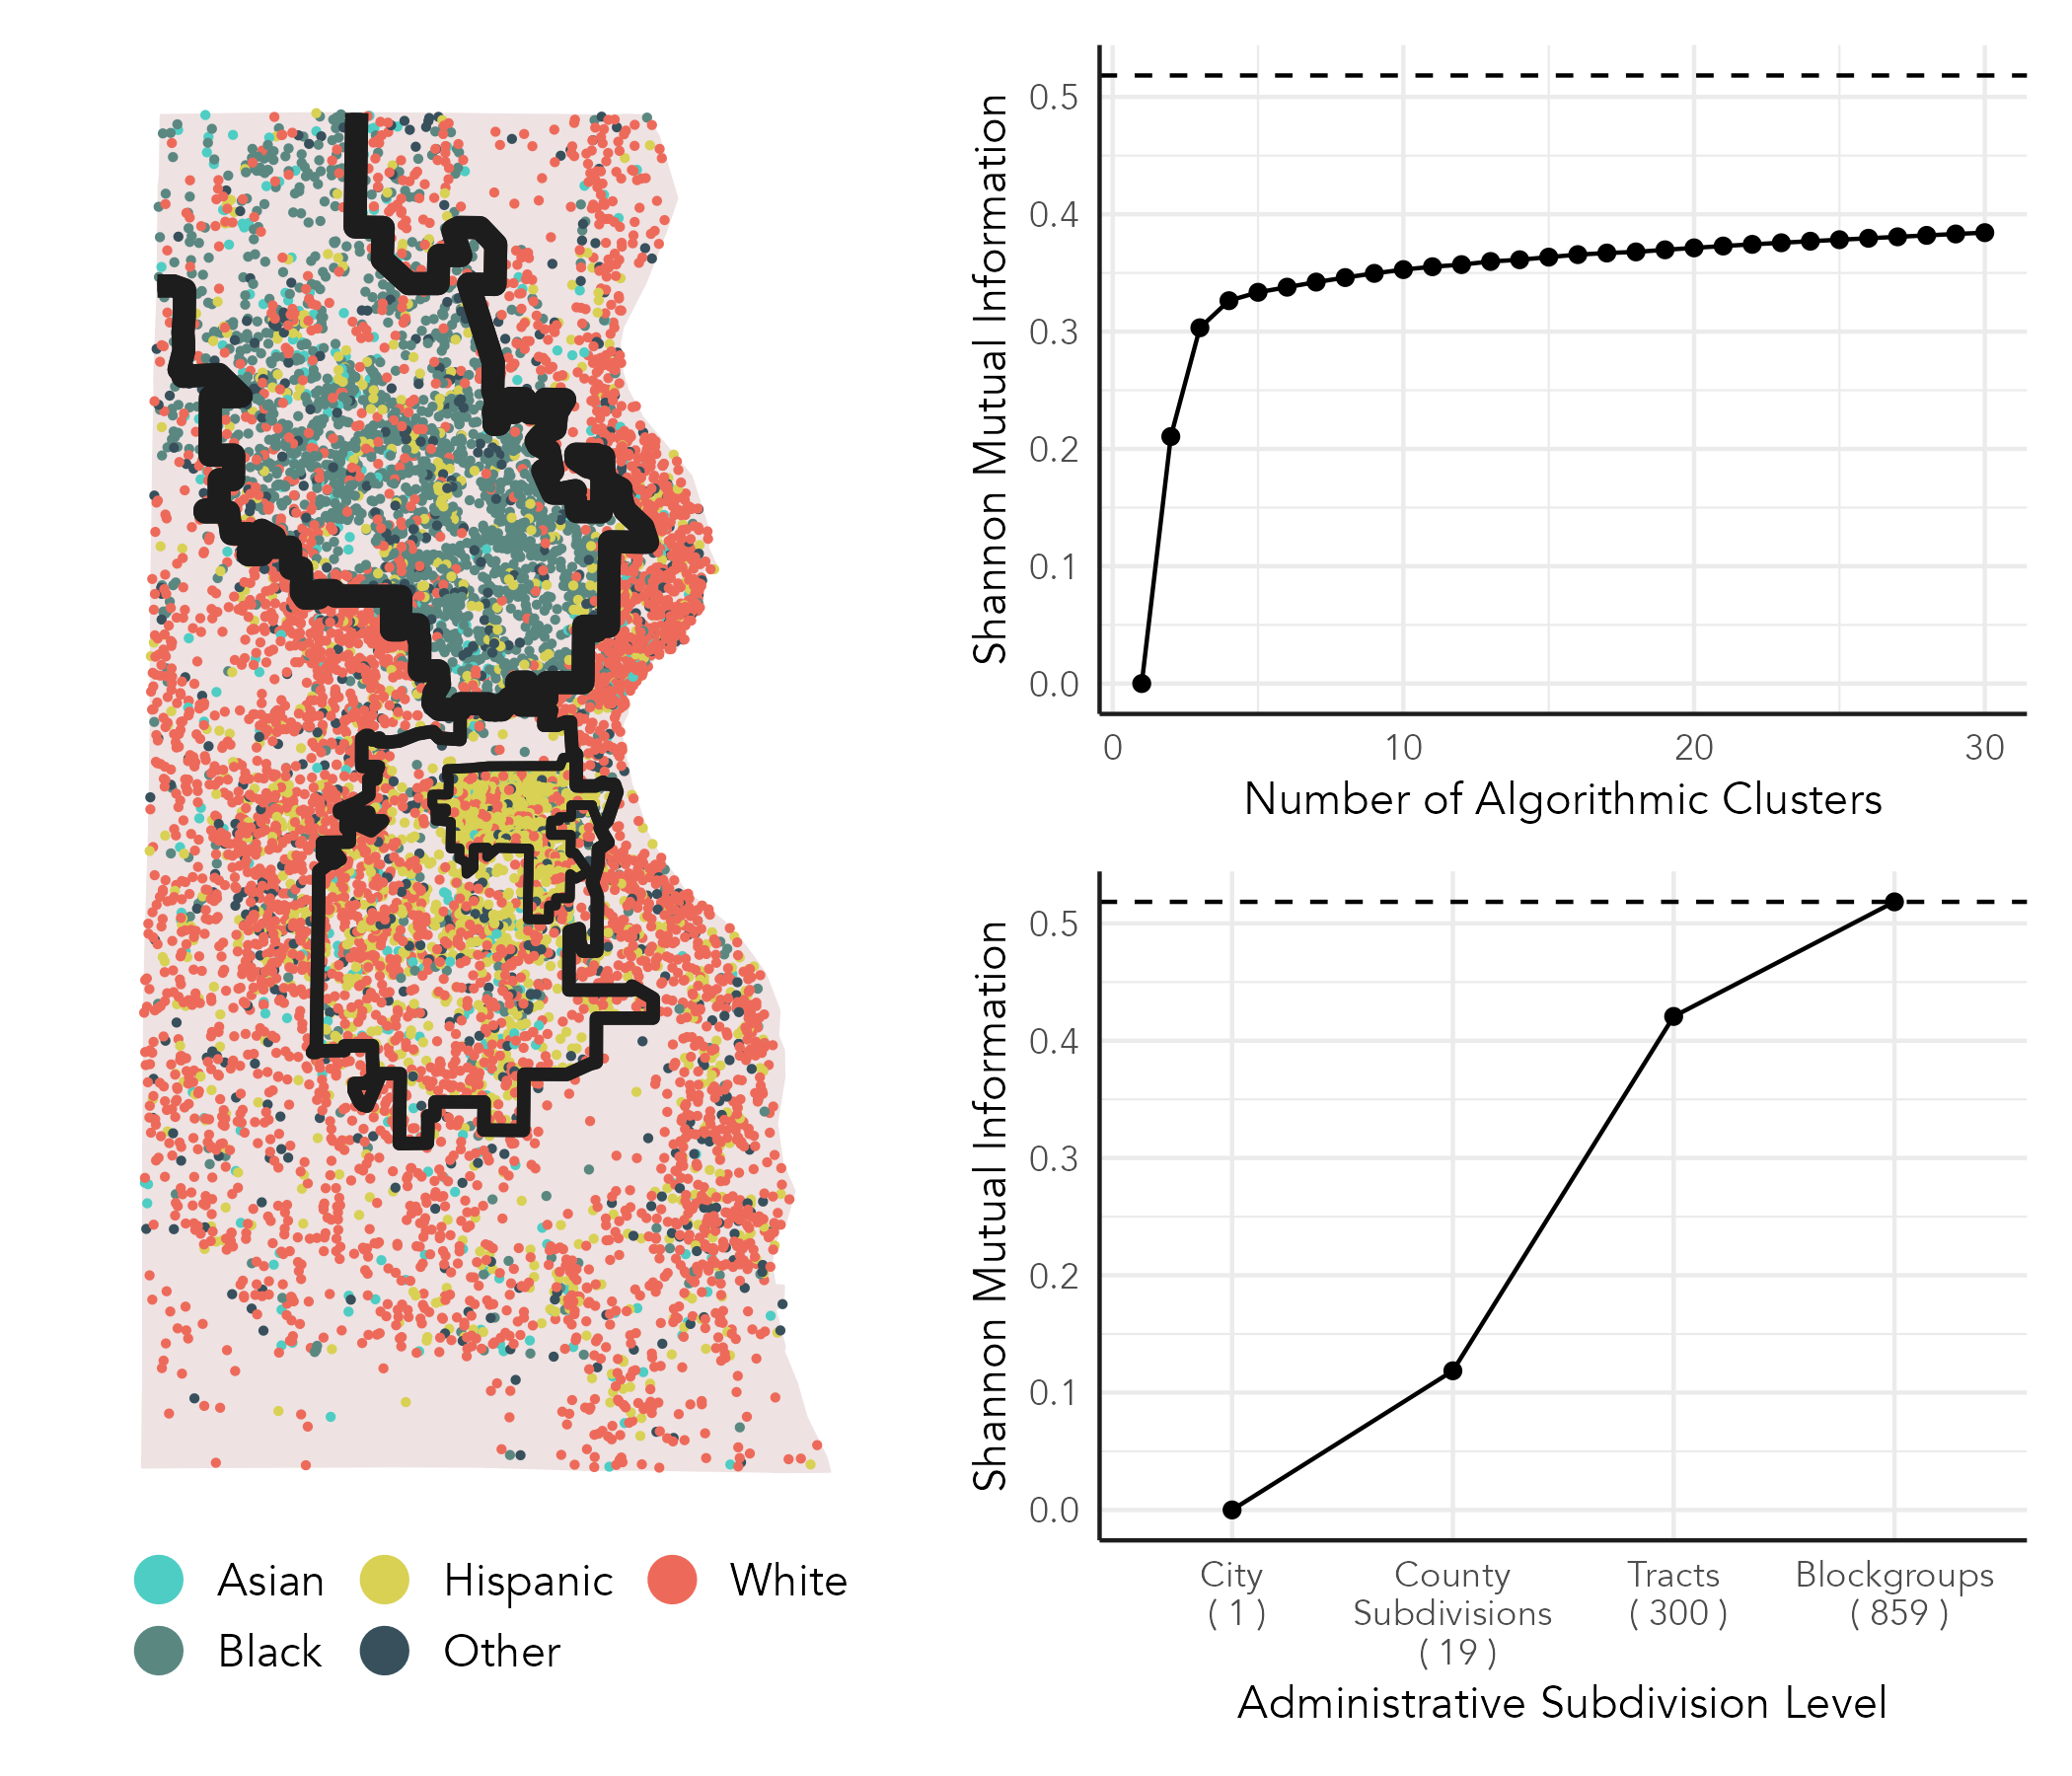
\includegraphics[width=0.5\textwidth]{fig/hclust-viz.png}
    \caption{Some caption.}
  \end{figure}

  \begin{figure}
    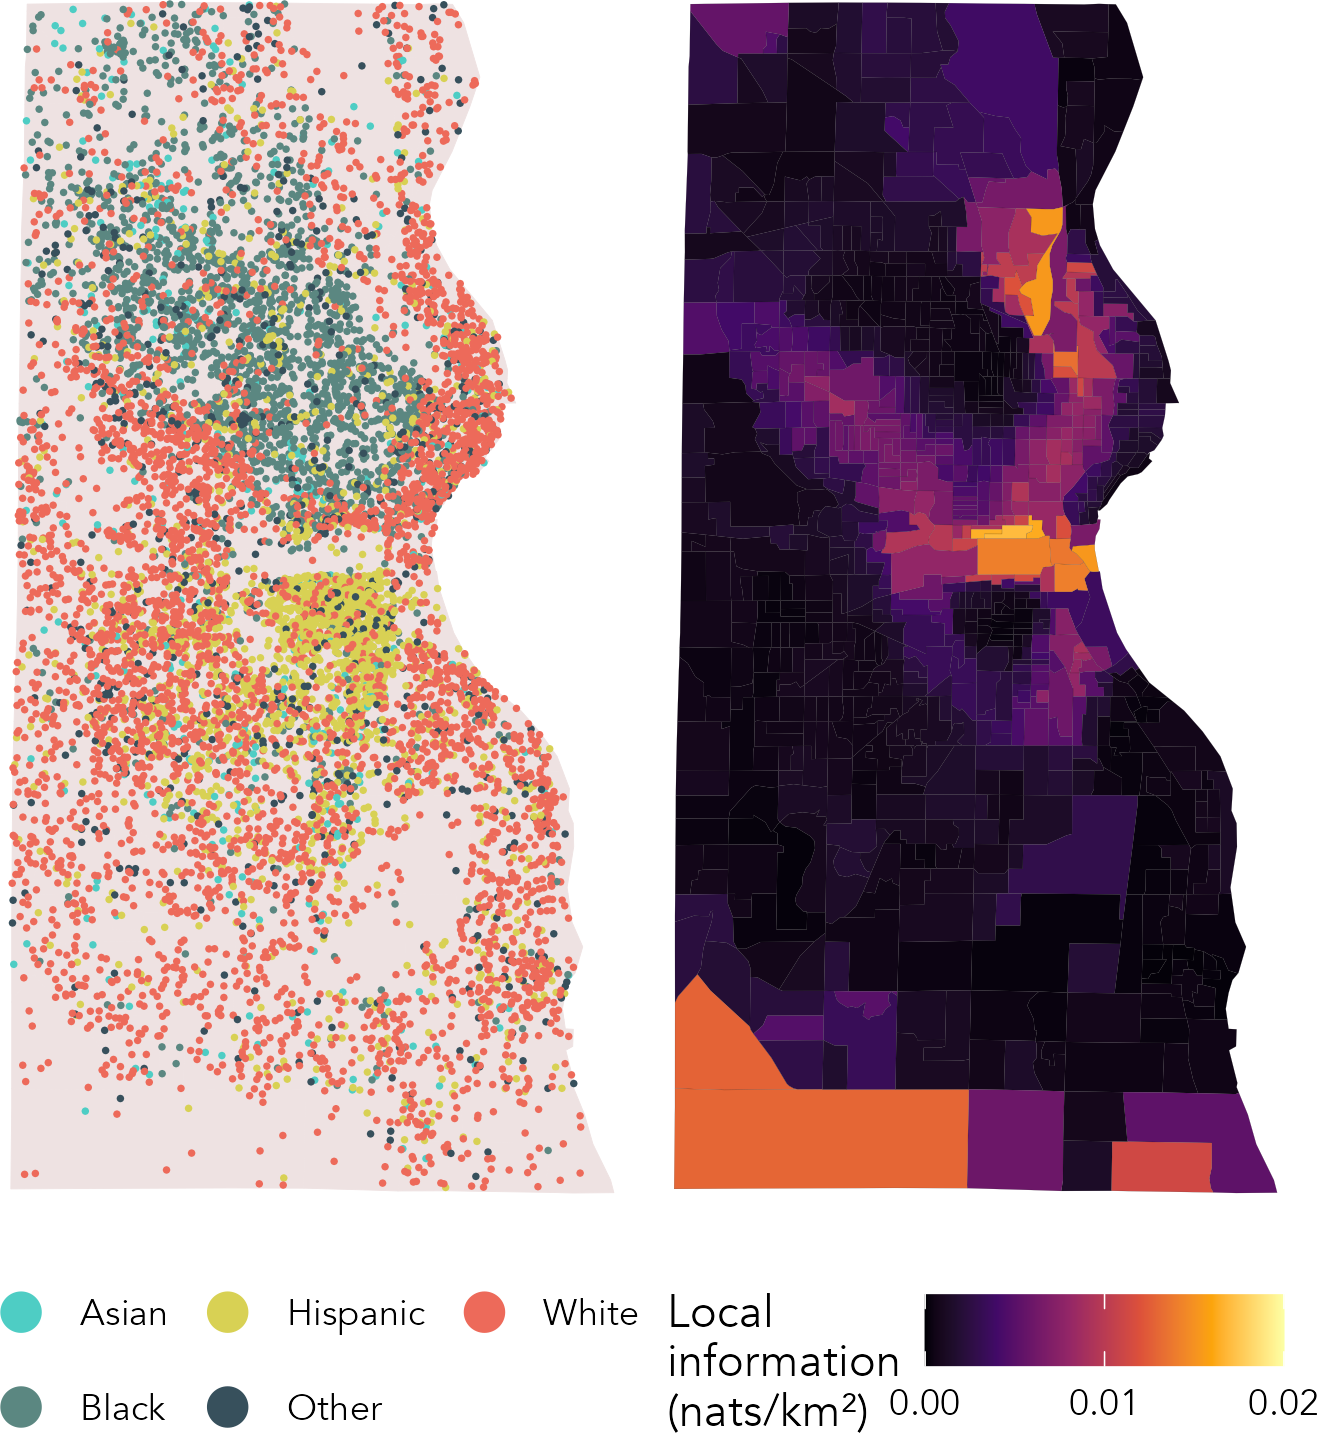
\includegraphics[width=0.5\textwidth]{fig/local-info.png}
    \caption{Another caption.}
  \end{figure}



  \subsection{Regionalization}
  \phil{Also bring in an example of generating a boundary via spatial aggregation.} 

  \subsection{Spatial Smoothing Kernels}

  \subsection{Local Information}

  \begin{dfn} \label{def:local-information}
    The local information!
  \end{dfn}

  \begin{thm}\label{thm:local-information}
    blah blah blah    
  \end{thm}









\section*{Extensions}

  Ordinal measures







\cite{chodrowEquivalenceInformationsCharacterizes2025b}
\cite{chodrowStructureInformationSpatial2017}

\cite{banerjeeClusteringBregmanDivergences2005}







\begin{figure}
  \centering
  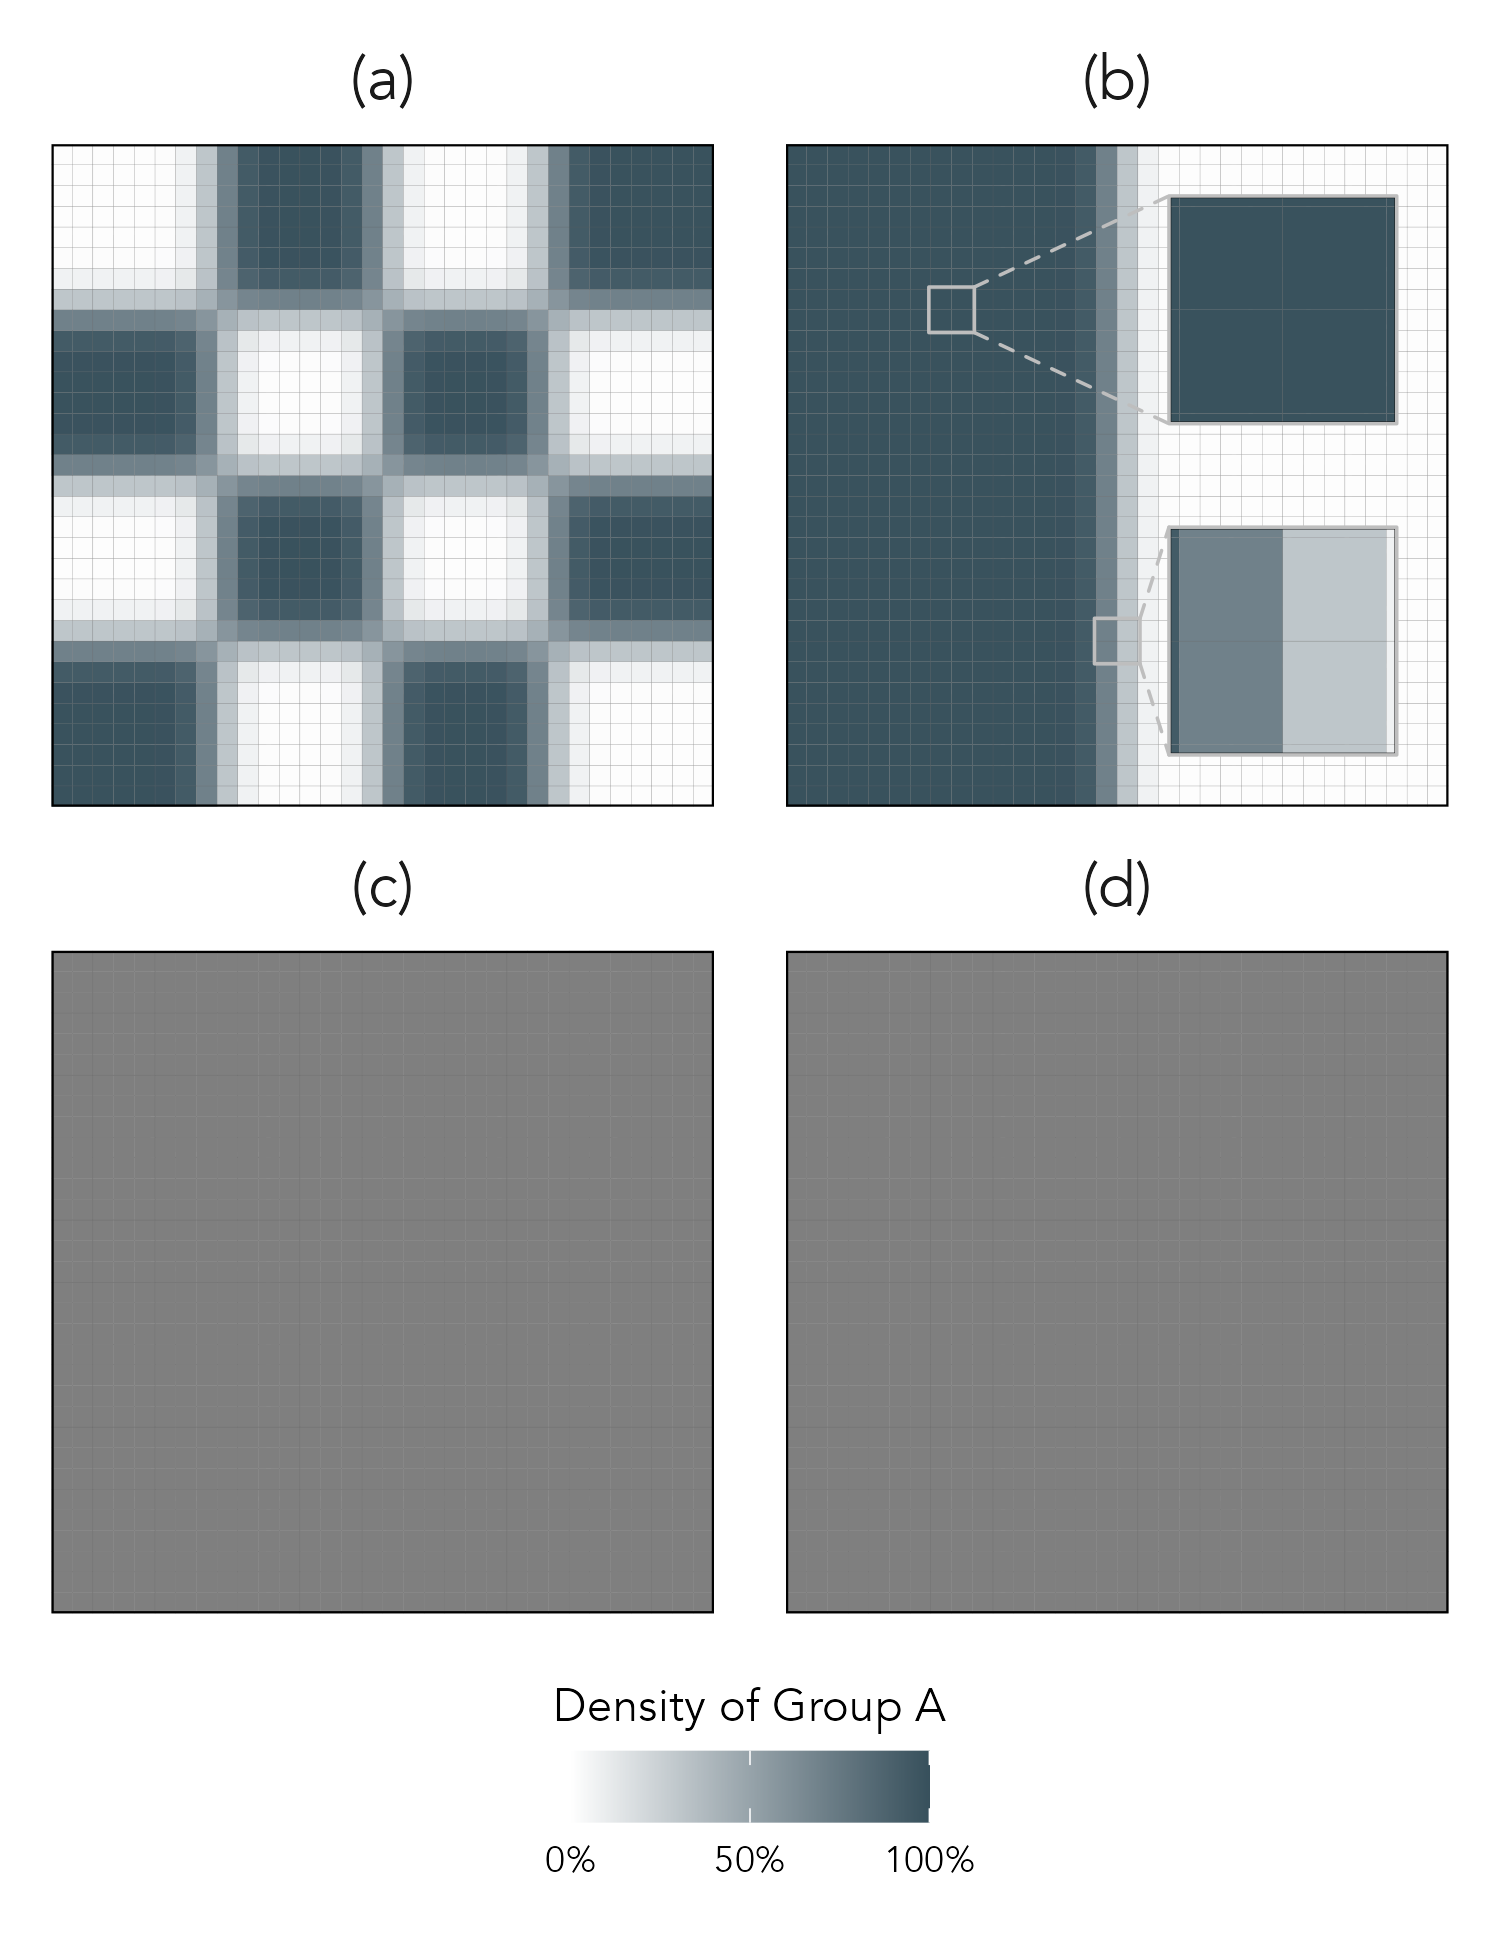
\includegraphics[width=0.5\textwidth]{fig/checkerboard-smoothed-and-trace.png}
  \caption{
    The smoothing bandwidth is $\smoothingBandwidth{}$ pixels. The mean local information of the checkerboard pattern is $\meanTraceChecker{}$, while the mean local information of the segregated pattern is $\meanTraceSeg{}$.
    } \label{fig:checkerboard-smoothed}
\end{figure}

\begin{figure*}
  \centering
  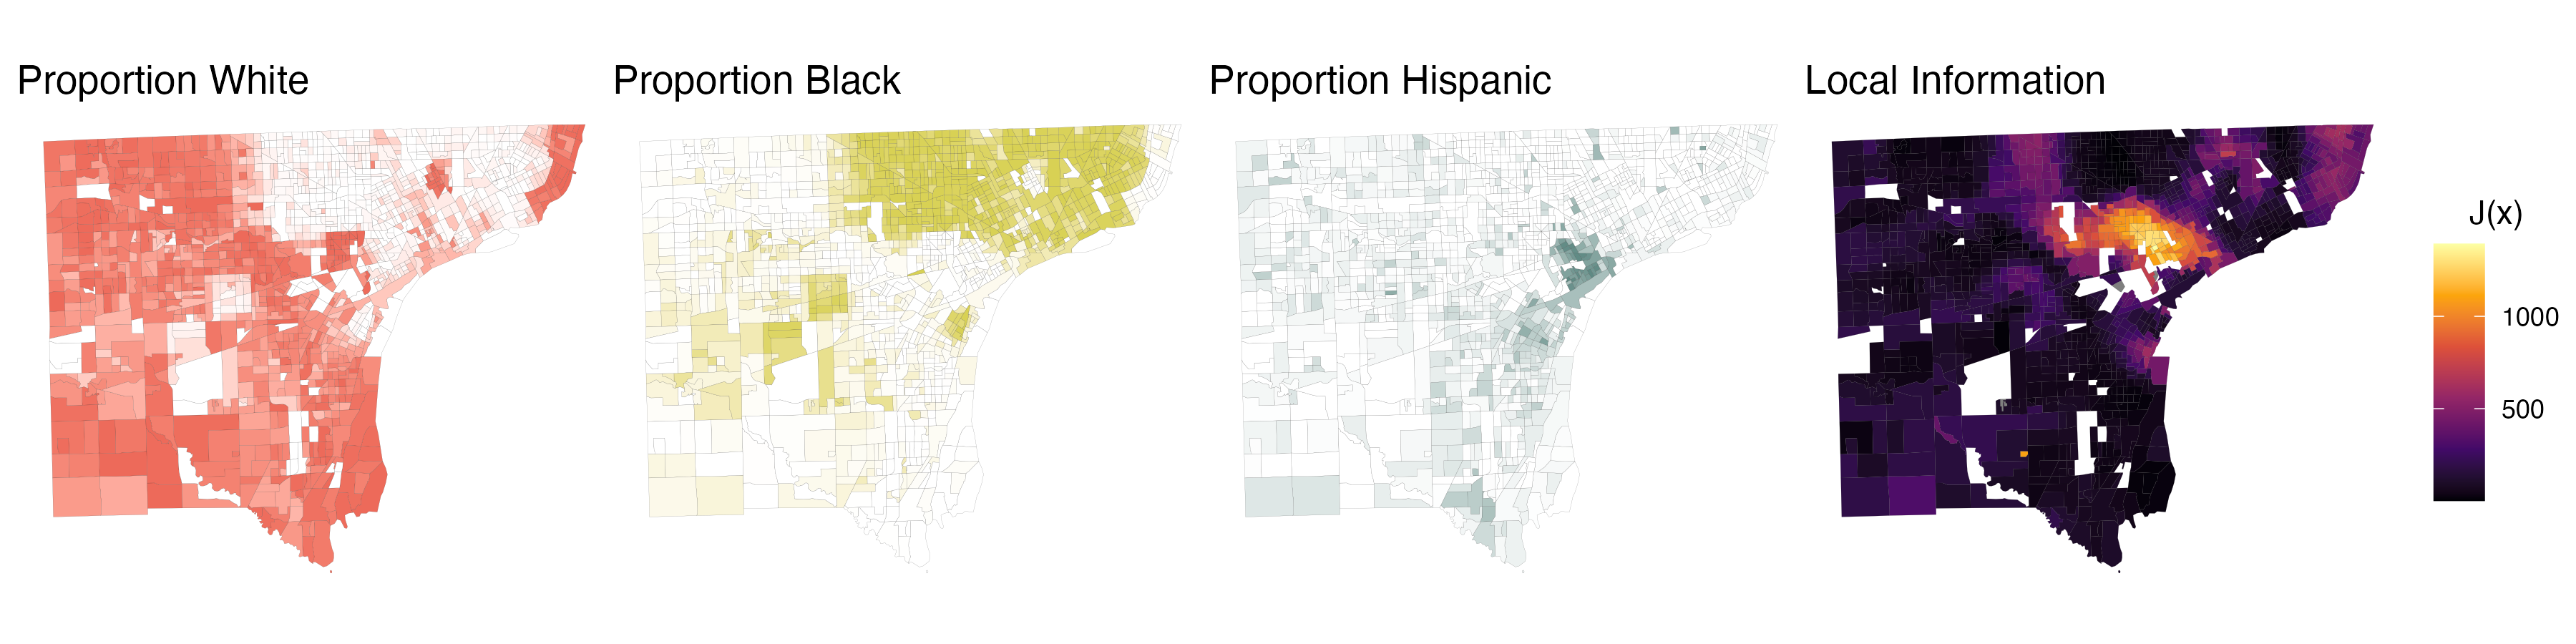
\includegraphics[width=1.0\textwidth]{fig/Detroit-local-info-overview.png}
  \caption{
    Test!!
    } \label{fig:city-local-info}
\end{figure*}

\begin{figure}
  \centering
  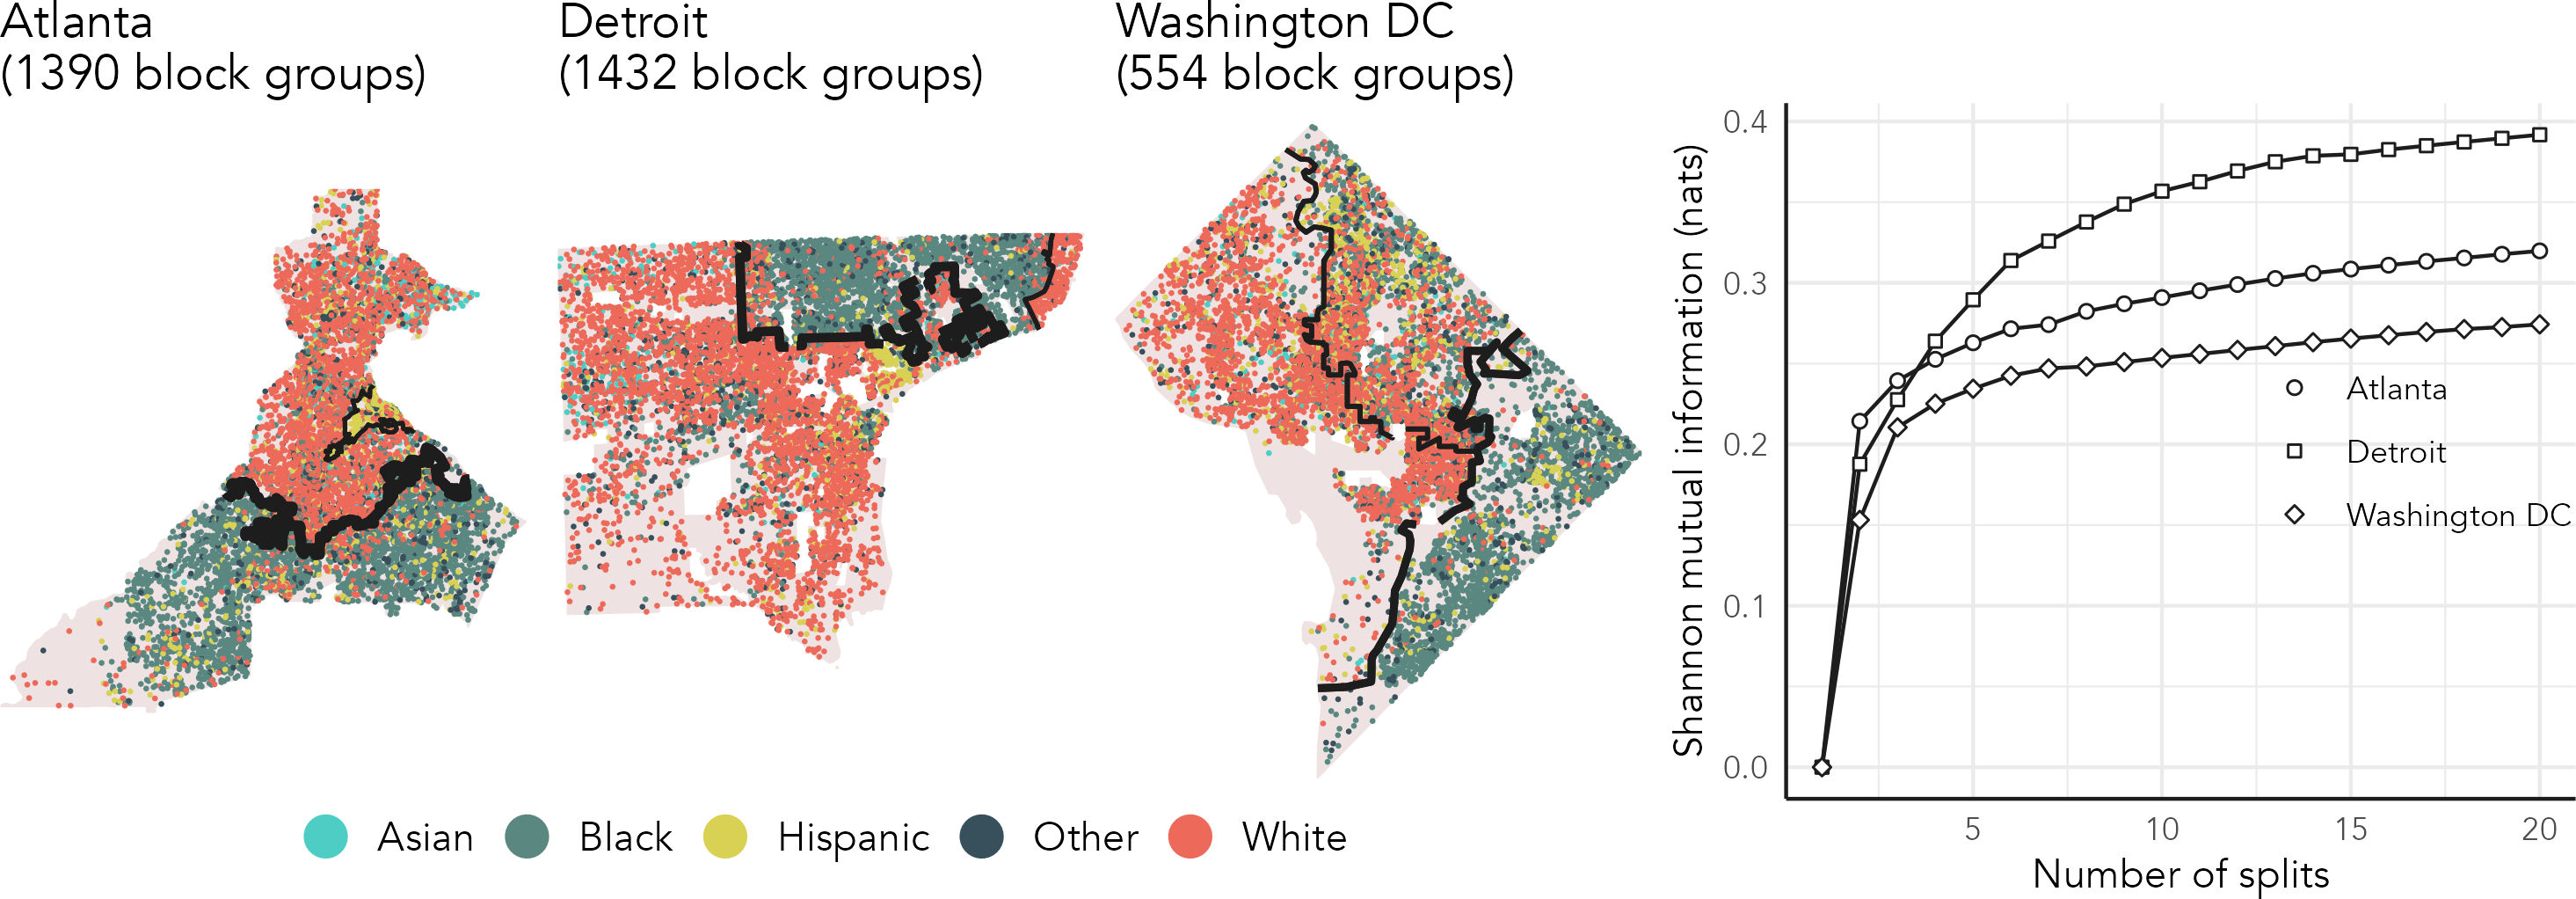
\includegraphics[width=0.5\textwidth]{fig/aggregation-viz.png}
  \caption{
    (Top): Heatmap showing the proportion of Black residents in \aggCity{}, delimited by nested areal units. 
    Thickest boundaries correspond to county subdivisions, thinner boundaries to Census tracts, and thinest boundaries to Census block groups.
    (Bottom): Behavior of the Shannon mutual information between Black and non-Black residents across geographic levels. 
    If $\cP$ is the population at the level of blockgroups (far left), the conditional Jensen information $I_\psi(\cP \mid \cP')$ is the difference between the given value of the information and the blockgroup value. 
    } \label{fig:aggregation-viz}
\end{figure}


%\bibliographystyle{foo}
\bibliography{refs}

\appendix 

\section{Supplementary Proofs}

\begin{proof}[Proof of \Cref{thm:monotone-under-group-addition}]
    \phil{This shouldn't require nonnegativity}
    Monotonicity under group addition is a consequence of convexity and nonnegativity: if $\psi$ is concave, then for any $I \subseteq [\ell]$ and $\lambda = \frac{|I|}{\ell}$, we have
    \begin{align*}
      \psi\paren{\frac{1}{\ell} \ve_{[\ell]} } 
      & = \psi\paren{\lambda \frac{1}{|I|} \ve_{I} + (1-\lambda) \frac{1}{\ell - |I|} \ve_{[\ell]\setminus I}} \\
      & \geq \lambda \psi\paren{\frac{1}{|I|} \ve_{I}} + (1-\lambda) \psi\paren{\frac{1}{\ell - |I|} \ve_{[\ell]\setminus I}} \\
      & \geq \psi\paren{\frac{1}{|I|} \ve_{I}} \;,
    \end{align*}
    where the first inequality is by convexity and the second is by nonnegativity. 
  \end{proof}

\begin{proof}[Proof of \Cref{thm:diversity-axioms-1}]
      To demonstrate maximization under the uniform, for any vector $\vy \in \simplex{\ell}$,
      \begin{align*}
        \ve_{[\ell]}/\ell = \frac{1}{\abs{\cS}}\sum_{\sigma \in \cS} \sigma(\vy) \;,
      \end{align*}
      where $\cS$ is the set of all permutations of $[\ell]$.
      It follows that 
      \begin{align*}
        \psi\paren{\frac{1}{\ell} \ve_{[\ell]}} 
        & = \psi\paren{\frac{1}{\abs{\cS}}\sum_{\sigma \in \cS} \sigma(\vy)} \\
        & < \frac{1}{\abs{\cS}}\sum_{\sigma \in \cS} \psi\paren{\sigma(\vy)} = \psi(\vy) \;,
      \end{align*}
      where the inequality is by an inductive application of strict concavity and the final equality is by symmetry.
  \end{proof}


\begin{proof}[Proof of \Cref{thm:exchanges}]
  The proof is by direct calculation. Let $\cP' = \exc{a}{b}{i}{j}{\epsilon}(\cP)$, and let $\vy_i'$ and $\vy_j'$ be the demographic vectors at locations $i$ and $j$ in $\cP'$. 
  Since the global demographic vector $\bar{\vy}$ is unchanged by the exchange, we have
  \begin{align*}
    I_{\psi}(\cP) - I_{\psi}(\cP') &= \sum_{i = 1}^n \brackets{\mu_i \psi(\vy_i) - \mu_i' \psi(\vy_i')} \\ 
    &= \mu_i\brackets{ \psi(\vy_i) - \psi(\vy_i')} + \mu_j\brackets{ \psi(\vy_j)  - \psi(\vy_j')} \\ 
    &= \mu_i \nabla \psi(\vy_i)^{\top} (\vy_i - \vy_i') \\ 
    & + \mu_j \nabla \psi(\vy_j)^{\top} (\vy_j - \vy_j') \\ 
    &+ o(\norm{\vy_i - \vy_i'}) + o(\norm{\vy_j - \vy_j'})\;. 
  \end{align*}
  since $\vy_k = \vy_k'$ for all $k \notin \{i, j\}$ and $\mu_k = \mu_k'$ for all $k$.
  Using now that $\vy_i - \vy_i' = \lambda_i (\tilde{\ve}_a - \tilde{\ve}_b)$ and $\vy_j - \vy_j' = \lambda_j (\tilde{\ve}_b - \tilde{\ve}_a)$ and ignoring the higher-order terms, we have 
  \begin{align*}
    I_{\psi}(\cP) - I_{\psi}(\cP') &\simeq \mu_i \lambda_i \nabla \psi(\vy_i)^{\top} (\tilde{\ve}_a - \tilde{\ve}_b) + \mu_j \lambda_j \nabla \psi(\vy_j)^{\top} (\tilde{\ve}_b - \tilde{\ve}_a)\;. 
  \end{align*}
  By the separability assumption, we have $\nabla \psi(\vy) = (\phi'(y_1), \ldots, \phi'(y_{\ell}))^{\top}$, and so 
  \begin{align*}
    I_{\psi}(\cP) - I_{\psi}(\cP') &\simeq \mu_i \lambda_i (\phi'(y_{ia}) - \phi'(y_{ib})) + \mu_j \lambda_j (\phi'(y_{jb}) - \phi'(y_{ja})) \\ 
    &= \epsilon (\phi'(y_{ia}) - \phi'(y_{ib}) + \phi'(y_{jb}) - \phi'(y_{ja})) \\ 
    &= \epsilon (\phi'(y_{ia}) - \phi'(y_{ja}) + \phi'(y_{jb}) - \phi'(y_{ib})) \\ 
    &> 0\;.
  \end{align*}
  The last line follows from the assumptions that $y_{ia} < y_{ja}$ and $y_{ib} > y_{jb}$, and the fact that, if $\phi$ is strictly convex, then $\phi'$ is strictly increasing, and so $\phi'(y_{ia}) - \phi'(y_{ja}) > 0$ and $\phi'(y_{jb}) - \phi'(y_{ib}) > 0$.
  Choosing $\epsilon*$ sufficiently small to justify the linear approximation completes the proof. 
\end{proof}



\section{Supplementary Exercises}

\begin{exercise}
    Give a heuristic justification for the convention that $0 \log 0 = 0$ by proving that $\lim_{x \rightarrow 0^+} x \log x = 0$.
\end{exercise}



\section*{Acknowledgements}

  I am grateful for support of the National Science Foundation's Division of Mathematical Sciences under award number DMS-2407058.

\section*{Software and Supplementary Information}

  Code sufficient to generate all figures from this article is available at \url{https://github.com/PhilChodrow/segregation-convexity}. 
  I used VSCode Copilot Pro for assistance in code generation. 
  Portions of the code were adapted from previous work \cite{chodrowStructureInformationSpatial2017}. 
  Supplementary information, including a discussion of Pielou's third axiom and several proofs, is available at \url{https://github.com/PhilChodrow/segregation-convexity/blob/main/supplementary.pdf}.

\bibliography{refs}



\end{document}

%%% Local Variables:
%%% mode: latex
%%% TeX-master: t
%%% End:
